% Options for packages loaded elsewhere
\PassOptionsToPackage{unicode}{hyperref}
\PassOptionsToPackage{hyphens}{url}
%
\documentclass[
]{article}
\title{incisionangles}
\author{Joao Marreiros}
\date{7/21/2021}

\usepackage{amsmath,amssymb}
\usepackage{lmodern}
\usepackage{iftex}
\ifPDFTeX
  \usepackage[T1]{fontenc}
  \usepackage[utf8]{inputenc}
  \usepackage{textcomp} % provide euro and other symbols
\else % if luatex or xetex
  \usepackage{unicode-math}
  \defaultfontfeatures{Scale=MatchLowercase}
  \defaultfontfeatures[\rmfamily]{Ligatures=TeX,Scale=1}
\fi
% Use upquote if available, for straight quotes in verbatim environments
\IfFileExists{upquote.sty}{\usepackage{upquote}}{}
\IfFileExists{microtype.sty}{% use microtype if available
  \usepackage[]{microtype}
  \UseMicrotypeSet[protrusion]{basicmath} % disable protrusion for tt fonts
}{}
\makeatletter
\@ifundefined{KOMAClassName}{% if non-KOMA class
  \IfFileExists{parskip.sty}{%
    \usepackage{parskip}
  }{% else
    \setlength{\parindent}{0pt}
    \setlength{\parskip}{6pt plus 2pt minus 1pt}}
}{% if KOMA class
  \KOMAoptions{parskip=half}}
\makeatother
\usepackage{xcolor}
\IfFileExists{xurl.sty}{\usepackage{xurl}}{} % add URL line breaks if available
\IfFileExists{bookmark.sty}{\usepackage{bookmark}}{\usepackage{hyperref}}
\hypersetup{
  pdftitle={incisionangles},
  pdfauthor={Joao Marreiros},
  hidelinks,
  pdfcreator={LaTeX via pandoc}}
\urlstyle{same} % disable monospaced font for URLs
\usepackage[margin=1in]{geometry}
\usepackage{color}
\usepackage{fancyvrb}
\newcommand{\VerbBar}{|}
\newcommand{\VERB}{\Verb[commandchars=\\\{\}]}
\DefineVerbatimEnvironment{Highlighting}{Verbatim}{commandchars=\\\{\}}
% Add ',fontsize=\small' for more characters per line
\usepackage{framed}
\definecolor{shadecolor}{RGB}{248,248,248}
\newenvironment{Shaded}{\begin{snugshade}}{\end{snugshade}}
\newcommand{\AlertTok}[1]{\textcolor[rgb]{0.94,0.16,0.16}{#1}}
\newcommand{\AnnotationTok}[1]{\textcolor[rgb]{0.56,0.35,0.01}{\textbf{\textit{#1}}}}
\newcommand{\AttributeTok}[1]{\textcolor[rgb]{0.77,0.63,0.00}{#1}}
\newcommand{\BaseNTok}[1]{\textcolor[rgb]{0.00,0.00,0.81}{#1}}
\newcommand{\BuiltInTok}[1]{#1}
\newcommand{\CharTok}[1]{\textcolor[rgb]{0.31,0.60,0.02}{#1}}
\newcommand{\CommentTok}[1]{\textcolor[rgb]{0.56,0.35,0.01}{\textit{#1}}}
\newcommand{\CommentVarTok}[1]{\textcolor[rgb]{0.56,0.35,0.01}{\textbf{\textit{#1}}}}
\newcommand{\ConstantTok}[1]{\textcolor[rgb]{0.00,0.00,0.00}{#1}}
\newcommand{\ControlFlowTok}[1]{\textcolor[rgb]{0.13,0.29,0.53}{\textbf{#1}}}
\newcommand{\DataTypeTok}[1]{\textcolor[rgb]{0.13,0.29,0.53}{#1}}
\newcommand{\DecValTok}[1]{\textcolor[rgb]{0.00,0.00,0.81}{#1}}
\newcommand{\DocumentationTok}[1]{\textcolor[rgb]{0.56,0.35,0.01}{\textbf{\textit{#1}}}}
\newcommand{\ErrorTok}[1]{\textcolor[rgb]{0.64,0.00,0.00}{\textbf{#1}}}
\newcommand{\ExtensionTok}[1]{#1}
\newcommand{\FloatTok}[1]{\textcolor[rgb]{0.00,0.00,0.81}{#1}}
\newcommand{\FunctionTok}[1]{\textcolor[rgb]{0.00,0.00,0.00}{#1}}
\newcommand{\ImportTok}[1]{#1}
\newcommand{\InformationTok}[1]{\textcolor[rgb]{0.56,0.35,0.01}{\textbf{\textit{#1}}}}
\newcommand{\KeywordTok}[1]{\textcolor[rgb]{0.13,0.29,0.53}{\textbf{#1}}}
\newcommand{\NormalTok}[1]{#1}
\newcommand{\OperatorTok}[1]{\textcolor[rgb]{0.81,0.36,0.00}{\textbf{#1}}}
\newcommand{\OtherTok}[1]{\textcolor[rgb]{0.56,0.35,0.01}{#1}}
\newcommand{\PreprocessorTok}[1]{\textcolor[rgb]{0.56,0.35,0.01}{\textit{#1}}}
\newcommand{\RegionMarkerTok}[1]{#1}
\newcommand{\SpecialCharTok}[1]{\textcolor[rgb]{0.00,0.00,0.00}{#1}}
\newcommand{\SpecialStringTok}[1]{\textcolor[rgb]{0.31,0.60,0.02}{#1}}
\newcommand{\StringTok}[1]{\textcolor[rgb]{0.31,0.60,0.02}{#1}}
\newcommand{\VariableTok}[1]{\textcolor[rgb]{0.00,0.00,0.00}{#1}}
\newcommand{\VerbatimStringTok}[1]{\textcolor[rgb]{0.31,0.60,0.02}{#1}}
\newcommand{\WarningTok}[1]{\textcolor[rgb]{0.56,0.35,0.01}{\textbf{\textit{#1}}}}
\usepackage{graphicx}
\makeatletter
\def\maxwidth{\ifdim\Gin@nat@width>\linewidth\linewidth\else\Gin@nat@width\fi}
\def\maxheight{\ifdim\Gin@nat@height>\textheight\textheight\else\Gin@nat@height\fi}
\makeatother
% Scale images if necessary, so that they will not overflow the page
% margins by default, and it is still possible to overwrite the defaults
% using explicit options in \includegraphics[width, height, ...]{}
\setkeys{Gin}{width=\maxwidth,height=\maxheight,keepaspectratio}
% Set default figure placement to htbp
\makeatletter
\def\fps@figure{htbp}
\makeatother
\setlength{\emergencystretch}{3em} % prevent overfull lines
\providecommand{\tightlist}{%
  \setlength{\itemsep}{0pt}\setlength{\parskip}{0pt}}
\setcounter{secnumdepth}{-\maxdimen} % remove section numbering
\usepackage{booktabs}
\usepackage{longtable}
\usepackage{array}
\usepackage{multirow}
\usepackage{wrapfig}
\usepackage{float}
\usepackage{colortbl}
\usepackage{pdflscape}
\usepackage{tabu}
\usepackage{threeparttable}
\usepackage{threeparttablex}
\usepackage[normalem]{ulem}
\usepackage{makecell}
\usepackage{xcolor}
\ifLuaTeX
  \usepackage{selnolig}  % disable illegal ligatures
\fi

\begin{document}
\maketitle

\textbf{Brief description of the script}

This R markdown document reads, summarizes and plots data concerning the
analysis of the Manot core engraved incisions, included in the
manuscript XXX.

The document contains:

\begin{enumerate}
\def\labelenumi{\arabic{enumi}.}
\tightlist
\item
  Tables
\item
  Figures (data analysis)
\end{enumerate}

This R project and respective scripts follow the procedures described by
Marwick et al.~2017.

To compile this markdown document do not delete or move files from their
original folders. Please note that most of the tables and figures in
this file do not match the numbering in the original manuscript.

For any questions, comments and inputs, please contact:

João Marreiros,
\href{mailto:marreiros@rgzm.de}{\nolinkurl{marreiros@rgzm.de}}

\hypertarget{load-data-into-r-project}{%
\section{Load data into R project}\label{load-data-into-r-project}}

\emph{Imported files are in: `../analysis/raw\_data'}

\emph{Figures are saved in: `../analysis/plots'}

\emph{Tables are saved in: `../analysis/derived\_data'}

\hypertarget{load-libraries}{%
\section{Load libraries}\label{load-libraries}}

\begin{Shaded}
\begin{Highlighting}[]
\FunctionTok{library}\NormalTok{(tidyverse)}
\end{Highlighting}
\end{Shaded}

\begin{verbatim}
## -- Attaching packages --------------------------------------- tidyverse 1.3.1 --
\end{verbatim}

\begin{verbatim}
## v ggplot2 3.3.5     v purrr   0.3.4
## v tibble  3.1.6     v dplyr   1.0.7
## v tidyr   1.1.4     v stringr 1.4.0
## v readr   2.1.1     v forcats 0.5.1
\end{verbatim}

\begin{verbatim}
## -- Conflicts ------------------------------------------ tidyverse_conflicts() --
## x dplyr::filter() masks stats::filter()
## x dplyr::lag()    masks stats::lag()
\end{verbatim}

\begin{Shaded}
\begin{Highlighting}[]
\FunctionTok{library}\NormalTok{(knitr)}
\FunctionTok{library}\NormalTok{(kableExtra)}
\end{Highlighting}
\end{Shaded}

\begin{verbatim}
## 
## Attaching package: 'kableExtra'
\end{verbatim}

\begin{verbatim}
## The following object is masked from 'package:dplyr':
## 
##     group_rows
\end{verbatim}

\begin{Shaded}
\begin{Highlighting}[]
\FunctionTok{library}\NormalTok{(GGally)}
\end{Highlighting}
\end{Shaded}

\begin{verbatim}
## Registered S3 method overwritten by 'GGally':
##   method from   
##   +.gg   ggplot2
\end{verbatim}

\begin{Shaded}
\begin{Highlighting}[]
\FunctionTok{library}\NormalTok{(doBy)}
\end{Highlighting}
\end{Shaded}

\begin{verbatim}
## 
## Attaching package: 'doBy'
\end{verbatim}

\begin{verbatim}
## The following object is masked from 'package:dplyr':
## 
##     order_by
\end{verbatim}

\begin{Shaded}
\begin{Highlighting}[]
\FunctionTok{library}\NormalTok{(ggfortify)}
\FunctionTok{library}\NormalTok{(tools)}
\FunctionTok{library}\NormalTok{(rstatix)}
\end{Highlighting}
\end{Shaded}

\begin{verbatim}
## 
## Attaching package: 'rstatix'
\end{verbatim}

\begin{verbatim}
## The following object is masked from 'package:stats':
## 
##     filter
\end{verbatim}

\begin{Shaded}
\begin{Highlighting}[]
\FunctionTok{library}\NormalTok{(ggpubr)}
\end{Highlighting}
\end{Shaded}

\hypertarget{import-dataset}{%
\section{Import dataset}\label{import-dataset}}

\begin{Shaded}
\begin{Highlighting}[]
\NormalTok{db }\OtherTok{\textless{}{-}} \FunctionTok{read\_csv}\NormalTok{(}\StringTok{"../raw\_data/incisionsangle.csv"}\NormalTok{, }\AttributeTok{na =} \FunctionTok{c}\NormalTok{(}\StringTok{""}\NormalTok{, }\StringTok{"NA"}\NormalTok{), }\AttributeTok{quoted\_na =} \ConstantTok{TRUE}\NormalTok{)}
\end{Highlighting}
\end{Shaded}

\begin{verbatim}
## Warning: The `quoted_na` argument of `read_csv()` is deprecated as of readr
## 2.0.0.
\end{verbatim}

\begin{verbatim}
## Rows: 114 Columns: 5
\end{verbatim}

\begin{verbatim}
## -- Column specification --------------------------------------------------------
## Delimiter: ","
## chr (1): site
## dbl (4): aoi, incision, angleid, angle
\end{verbatim}

\begin{verbatim}
## 
## i Use `spec()` to retrieve the full column specification for this data.
## i Specify the column types or set `show_col_types = FALSE` to quiet this message.
\end{verbatim}

\begin{Shaded}
\begin{Highlighting}[]
\NormalTok{data\_file }\OtherTok{\textless{}{-}} \FunctionTok{list.files}\NormalTok{(}\StringTok{"../raw\_data/"}\NormalTok{, }\AttributeTok{pattern =} \StringTok{"}\SpecialCharTok{\textbackslash{}\textbackslash{}}\StringTok{.csv$"}\NormalTok{, }\AttributeTok{full.names =} \ConstantTok{TRUE}\NormalTok{)}
\end{Highlighting}
\end{Shaded}

Show dataset:

\begin{Shaded}
\begin{Highlighting}[]
\FunctionTok{str}\NormalTok{(db)}
\end{Highlighting}
\end{Shaded}

\begin{verbatim}
## spec_tbl_df [114 x 5] (S3: spec_tbl_df/tbl_df/tbl/data.frame)
##  $ site    : chr [1:114] "Manot" "Manot" "Manot" "Manot" ...
##  $ aoi     : num [1:114] 1 1 1 1 1 1 1 1 1 1 ...
##  $ incision: num [1:114] 4 6 6 6 5 5 4 5 8 4 ...
##  $ angleid : num [1:114] 1 2 3 4 5 6 7 8 9 10 ...
##  $ angle   : num [1:114] 168 162 168 158 165 ...
##  - attr(*, "spec")=
##   .. cols(
##   ..   site = col_character(),
##   ..   aoi = col_double(),
##   ..   incision = col_double(),
##   ..   angleid = col_double(),
##   ..   angle = col_double()
##   .. )
##  - attr(*, "problems")=<externalptr>
\end{verbatim}

\hypertarget{import-and-summarize-data}{%
\section{Import and summarize data}\label{import-and-summarize-data}}

\begin{Shaded}
\begin{Highlighting}[]
\CommentTok{\# compute descriptive statistics}

\NormalTok{nminmaxmeanmedsd }\OtherTok{\textless{}{-}} \ControlFlowTok{function}\NormalTok{(x)\{}
\NormalTok{    y }\OtherTok{\textless{}{-}}\NormalTok{ x[}\SpecialCharTok{!}\FunctionTok{is.na}\NormalTok{(x)]}
\NormalTok{    n\_test }\OtherTok{\textless{}{-}} \FunctionTok{length}\NormalTok{(y)}
\NormalTok{    min\_test }\OtherTok{\textless{}{-}} \FunctionTok{min}\NormalTok{(y)}
\NormalTok{    max\_test }\OtherTok{\textless{}{-}} \FunctionTok{max}\NormalTok{(y)}
\NormalTok{    mean\_test }\OtherTok{\textless{}{-}} \FunctionTok{mean}\NormalTok{(y)}
\NormalTok{    med\_test }\OtherTok{\textless{}{-}} \FunctionTok{median}\NormalTok{(y)}
\NormalTok{    sd\_test }\OtherTok{\textless{}{-}} \FunctionTok{sd}\NormalTok{(y)}
\NormalTok{    out }\OtherTok{\textless{}{-}} \FunctionTok{c}\NormalTok{(n\_test, min\_test, max\_test, mean\_test, med\_test, sd\_test)}
    \FunctionTok{names}\NormalTok{(out) }\OtherTok{\textless{}{-}} \FunctionTok{c}\NormalTok{(}\StringTok{"n"}\NormalTok{, }\StringTok{"min"}\NormalTok{, }\StringTok{"max"}\NormalTok{, }\StringTok{"mean"}\NormalTok{, }\StringTok{"median"}\NormalTok{, }\StringTok{"sd"}\NormalTok{)}
    \FunctionTok{return}\NormalTok{(out)}
\NormalTok{\}}

\NormalTok{num.var }\OtherTok{\textless{}{-}} \DecValTok{5}\SpecialCharTok{:}\FunctionTok{length}\NormalTok{(db)}

\NormalTok{anglestats }\OtherTok{\textless{}{-}} \FunctionTok{summaryBy}\NormalTok{(.}\SpecialCharTok{\textasciitilde{}}\NormalTok{aoi }\SpecialCharTok{+}\NormalTok{ site }\SpecialCharTok{+}\NormalTok{ incision, }\AttributeTok{data=}\NormalTok{db[}\FunctionTok{c}\NormalTok{(}\StringTok{"site"}\NormalTok{, }\StringTok{"incision"}\NormalTok{, }\FunctionTok{names}\NormalTok{(db)[num.var])], }\AttributeTok{FUN=}\NormalTok{nminmaxmeanmedsd)}

\NormalTok{anglestats}
\end{Highlighting}
\end{Shaded}

\begin{verbatim}
## # A tibble: 25 x 8
##    site   incision angle.n angle.min angle.max angle.mean angle.median angle.sd
##    <chr>     <dbl>   <dbl>     <dbl>     <dbl>      <dbl>        <dbl>    <dbl>
##  1 Manot         1      12      148.      168.       156.         158.     5.86
##  2 Manot         2       7      153.      171.       164.         168.     7.07
##  3 Manot         3       3      146.      164.       156.         159.     9.27
##  4 Manot         4       7      156.      168.       163.         163.     4.81
##  5 Manot         5       3      162.      168.       165.         165.     2.99
##  6 Manot         6       3      158.      168.       162.         162.     5.11
##  7 Manot         7       1      152.      152.       152.         152.    NA   
##  8 Manot         8       1      166.      166.       166.         166.    NA   
##  9 Qafzeh        1       1      154.      154.       154.         154.    NA   
## 10 Qafzeh        2       2      160.      165.       163.         163.     3.64
## # ... with 15 more rows
\end{verbatim}

\begin{Shaded}
\begin{Highlighting}[]
\FunctionTok{write\_csv}\NormalTok{(anglestats, }\StringTok{"../summary\_stats/anglestats.csv"}\NormalTok{)}
\end{Highlighting}
\end{Shaded}

\hypertarget{plot-data}{%
\section{Plot data}\label{plot-data}}

\begin{Shaded}
\begin{Highlighting}[]
\CommentTok{\# converting to categorical}
\NormalTok{db}\SpecialCharTok{$}\NormalTok{aoi }\OtherTok{=} \FunctionTok{as.factor}\NormalTok{(db}\SpecialCharTok{$}\NormalTok{aoi) }
\CommentTok{\# db$incision = as.factor(db$incision)}

\NormalTok{sitesangle }\OtherTok{\textless{}{-}} \FunctionTok{ggplot}\NormalTok{(}\AttributeTok{data =}\NormalTok{ db, }\FunctionTok{aes}\NormalTok{(}\AttributeTok{x =}\NormalTok{ site, }\AttributeTok{y =}\NormalTok{ angle)) }\SpecialCharTok{+}  
           \FunctionTok{geom\_boxplot}\NormalTok{() }\SpecialCharTok{+}
           \FunctionTok{theme\_bw}\NormalTok{()}\SpecialCharTok{+}\FunctionTok{scale\_fill\_grey}\NormalTok{(}\AttributeTok{start =} \FloatTok{0.8}\NormalTok{, }\AttributeTok{end =} \DecValTok{1}\NormalTok{) }\SpecialCharTok{+}
           \FunctionTok{labs}\NormalTok{( }\AttributeTok{x =} \StringTok{""}\NormalTok{, }\AttributeTok{y =} \StringTok{"Angle in º"}\NormalTok{) }\SpecialCharTok{+}
           \FunctionTok{geom\_jitter}\NormalTok{(}\FunctionTok{aes}\NormalTok{(}\AttributeTok{colour =}\NormalTok{ site), }\AttributeTok{alpha=}\FloatTok{0.9}\NormalTok{, }\AttributeTok{position=}\FunctionTok{position\_jitter}\NormalTok{(}\AttributeTok{w=}\FloatTok{0.1}\NormalTok{,}\AttributeTok{h=}\FloatTok{0.1}\NormalTok{))}

\FunctionTok{print}\NormalTok{(sitesangle)}
\end{Highlighting}
\end{Shaded}

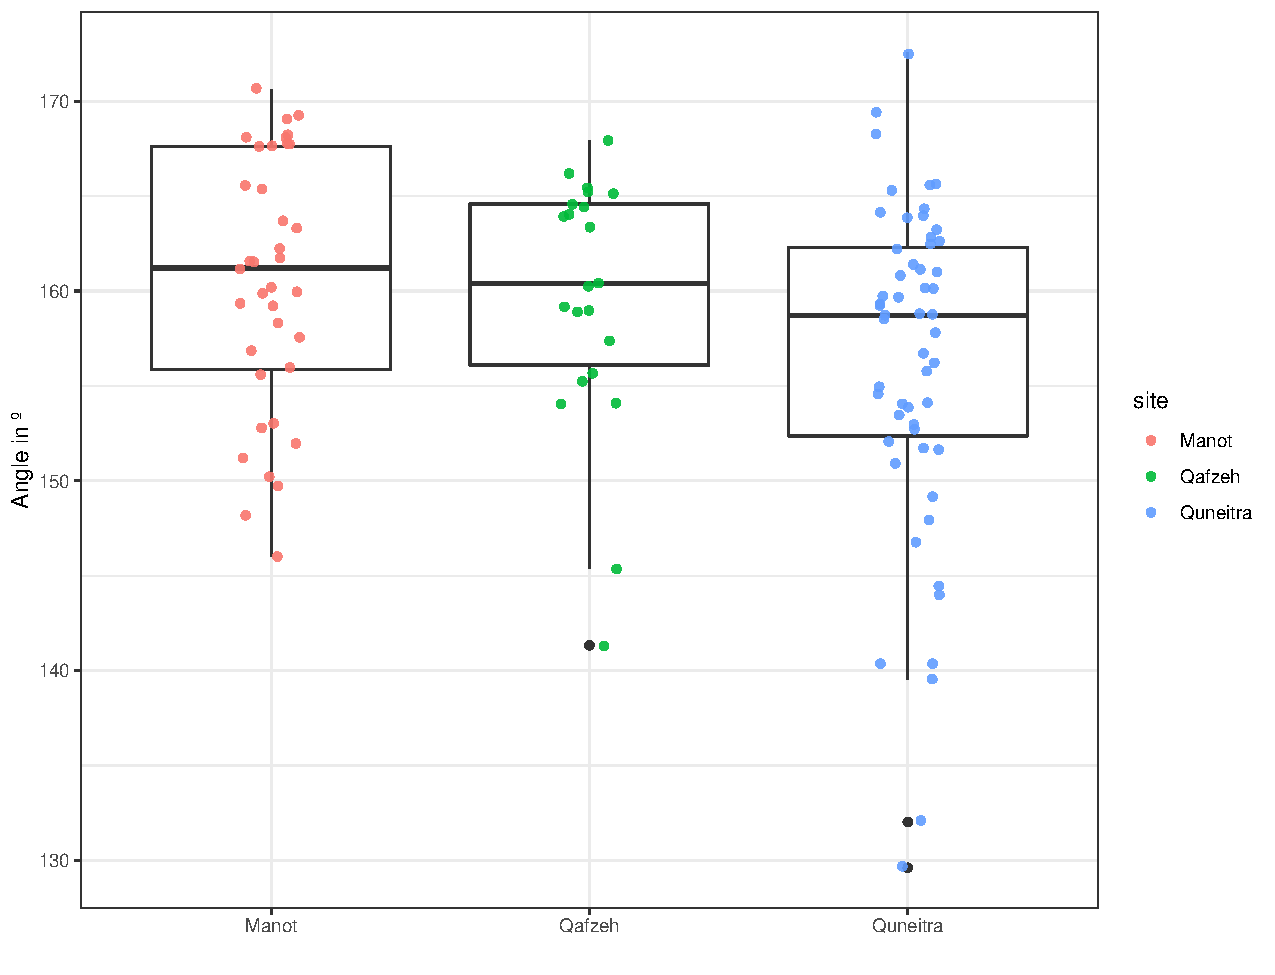
\includegraphics{incisionangles_files/figure-latex/unnamed-chunk-5-1.pdf}

\begin{Shaded}
\begin{Highlighting}[]
\FunctionTok{ggsave}\NormalTok{(}\StringTok{"../plots/sitesangle.png"}\NormalTok{)}
\end{Highlighting}
\end{Shaded}

\begin{verbatim}
## Saving 8.5 x 6.5 in image
\end{verbatim}

\hypertarget{run-anova-for-comparison}{%
\section{Run ANOVA for comparison}\label{run-anova-for-comparison}}

\begin{Shaded}
\begin{Highlighting}[]
\CommentTok{\# brief visualization of the data from the 3 artifacts}

\FunctionTok{ggplot}\NormalTok{(}\AttributeTok{data =}\NormalTok{ db, }\FunctionTok{aes}\NormalTok{(}\AttributeTok{x=}\NormalTok{ site, }\AttributeTok{y=}\NormalTok{ angle)) }\SpecialCharTok{+}
  \FunctionTok{geom\_boxplot}\NormalTok{()}
\end{Highlighting}
\end{Shaded}

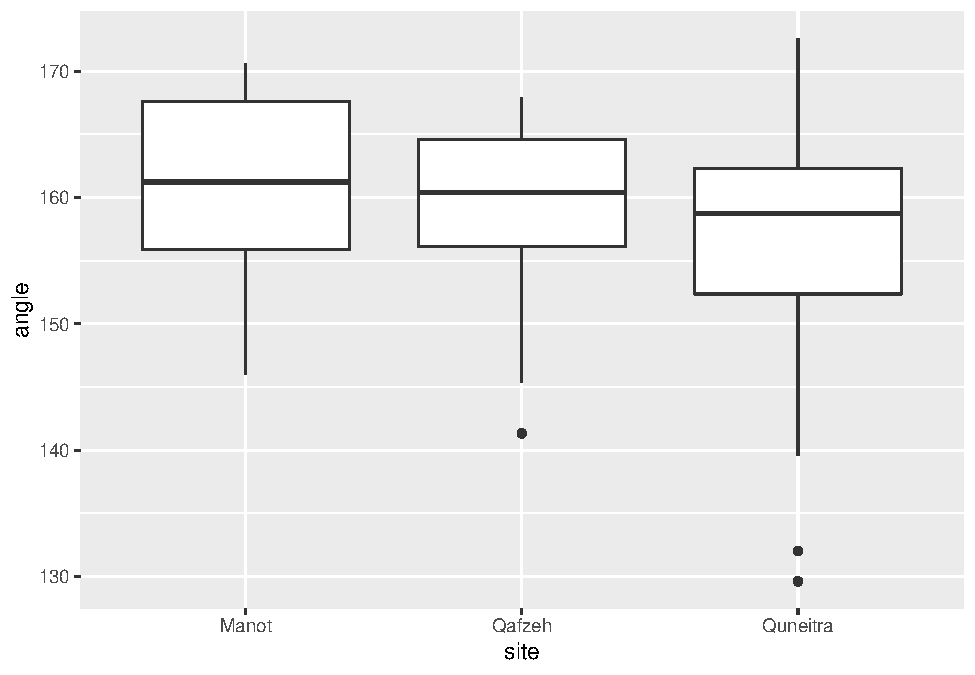
\includegraphics{incisionangles_files/figure-latex/unnamed-chunk-6-1.pdf}

\begin{Shaded}
\begin{Highlighting}[]
\CommentTok{\# check for outliers}

\NormalTok{db }\SpecialCharTok{\%\textgreater{}\%}
  \FunctionTok{group\_by}\NormalTok{(site) }\SpecialCharTok{\%\textgreater{}\%}
  \FunctionTok{identify\_outliers}\NormalTok{(angle)}
\end{Highlighting}
\end{Shaded}

\begin{verbatim}
## # A tibble: 3 x 7
##   site     aoi   incision angleid angle is.outlier is.extreme
##   <chr>    <fct>    <dbl>   <dbl> <dbl> <lgl>      <lgl>     
## 1 Qafzeh   1           10       1  141. TRUE       FALSE     
## 2 Quneitra 2            2       2  132. TRUE       FALSE     
## 3 Quneitra 2            7      32  130. TRUE       FALSE
\end{verbatim}

\begin{Shaded}
\begin{Highlighting}[]
\CommentTok{\# there are no extreme outliers}

\CommentTok{\# check normality}

\NormalTok{model }\OtherTok{\textless{}{-}} \FunctionTok{lm}\NormalTok{(angle }\SpecialCharTok{\textasciitilde{}}\NormalTok{ site, }\AttributeTok{data =}\NormalTok{ db)}

\CommentTok{\# QQ plot of residuals}

\FunctionTok{ggqqplot}\NormalTok{(}\FunctionTok{residuals}\NormalTok{(model))}
\end{Highlighting}
\end{Shaded}

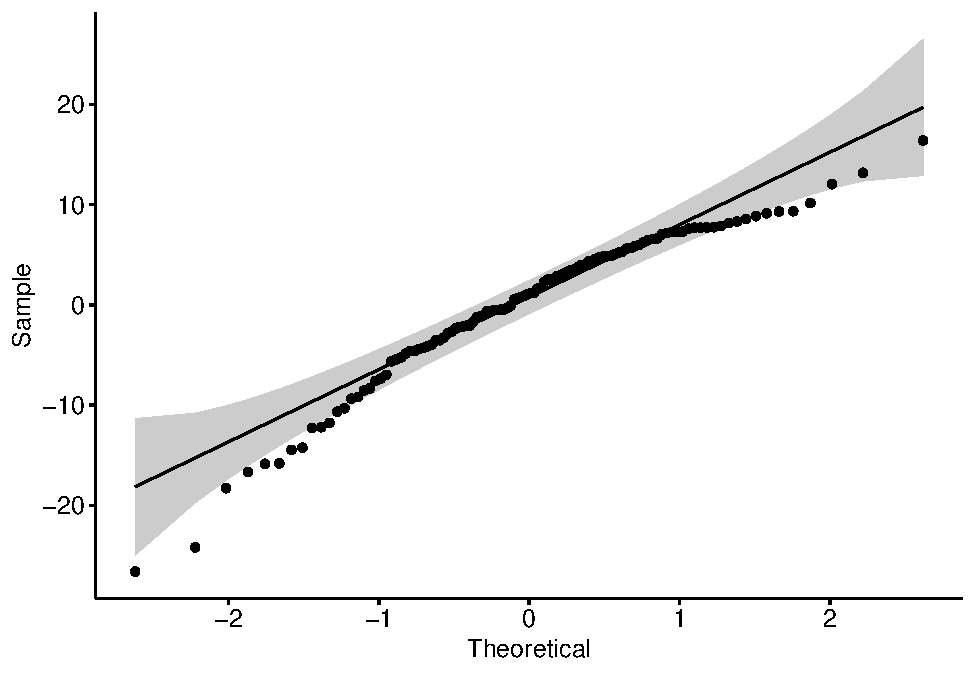
\includegraphics{incisionangles_files/figure-latex/unnamed-chunk-6-2.pdf}

\begin{Shaded}
\begin{Highlighting}[]
\FunctionTok{shapiro\_test}\NormalTok{(}\FunctionTok{residuals}\NormalTok{(model))}
\end{Highlighting}
\end{Shaded}

\begin{verbatim}
## # A tibble: 1 x 3
##   variable         statistic  p.value
##   <chr>                <dbl>    <dbl>
## 1 residuals(model)     0.947 0.000198
\end{verbatim}

\begin{Shaded}
\begin{Highlighting}[]
\NormalTok{db }\SpecialCharTok{\%\textgreater{}\%}
  \FunctionTok{group\_by}\NormalTok{(site) }\SpecialCharTok{\%\textgreater{}\%}
  \FunctionTok{shapiro\_test}\NormalTok{(angle)}
\end{Highlighting}
\end{Shaded}

\begin{verbatim}
## # A tibble: 3 x 4
##   site     variable statistic       p
##   <chr>    <chr>        <dbl>   <dbl>
## 1 Manot    angle        0.949 0.0893 
## 2 Qafzeh   angle        0.876 0.0101 
## 3 Quneitra angle        0.934 0.00483
\end{verbatim}

\begin{Shaded}
\begin{Highlighting}[]
\FunctionTok{ggqqplot}\NormalTok{(db, }\StringTok{"angle"}\NormalTok{, }\AttributeTok{facet.by =} \StringTok{"site"}\NormalTok{)}
\end{Highlighting}
\end{Shaded}

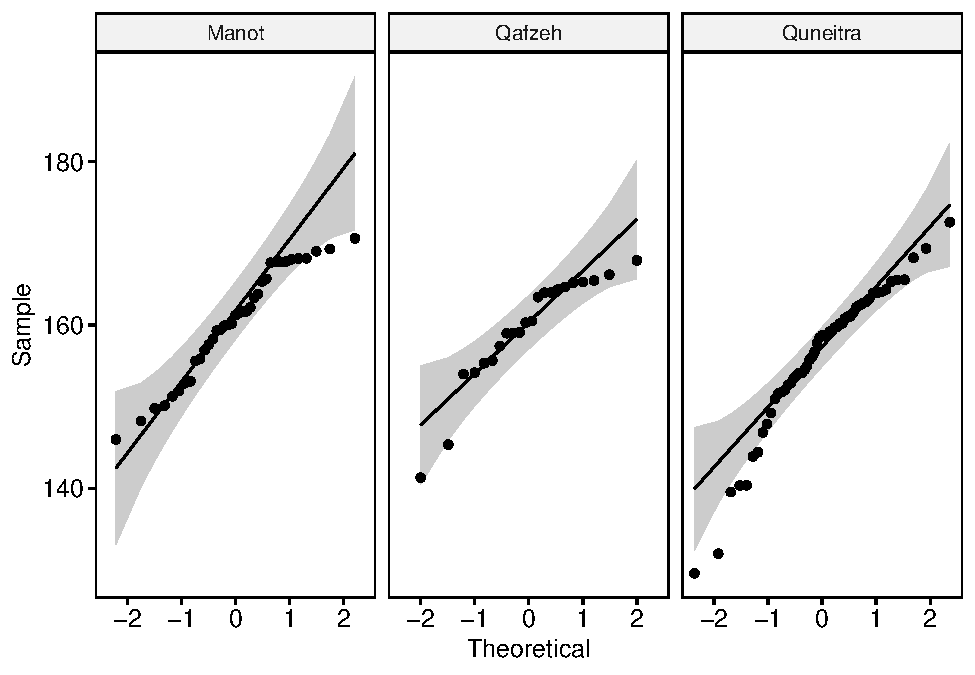
\includegraphics{incisionangles_files/figure-latex/unnamed-chunk-6-3.pdf}

\begin{Shaded}
\begin{Highlighting}[]
\NormalTok{ang.aov }\OtherTok{\textless{}{-}}\NormalTok{ db }\SpecialCharTok{\%\textgreater{}\%} \FunctionTok{anova\_test}\NormalTok{(angle }\SpecialCharTok{\textasciitilde{}}\NormalTok{ site)}
\end{Highlighting}
\end{Shaded}

\begin{verbatim}
## Coefficient covariances computed by hccm()
\end{verbatim}

\begin{Shaded}
\begin{Highlighting}[]
\NormalTok{ang.aov}
\end{Highlighting}
\end{Shaded}

\begin{verbatim}
## ANOVA Table (type II tests)
## 
##   Effect DFn DFd     F     p p<.05   ges
## 1   site   2 111 3.686 0.028     * 0.062
\end{verbatim}

\begin{Shaded}
\begin{Highlighting}[]
\CommentTok{\# post{-}hoc test}

\NormalTok{ang.pwc }\OtherTok{\textless{}{-}}\NormalTok{ db }\SpecialCharTok{\%\textgreater{}\%} \FunctionTok{tukey\_hsd}\NormalTok{(angle }\SpecialCharTok{\textasciitilde{}}\NormalTok{ site)}
\NormalTok{ang.pwc}
\end{Highlighting}
\end{Shaded}

\begin{verbatim}
## # A tibble: 3 x 9
##   term  group1 group2 null.value estimate conf.low conf.high  p.adj p.adj.signif
## * <chr> <chr>  <chr>       <dbl>    <dbl>    <dbl>     <dbl>  <dbl> <chr>       
## 1 site  Manot  Qafzeh          0   -0.844    -5.84     4.16  0.915  ns          
## 2 site  Manot  Qunei~          0   -4.25     -8.20    -0.301 0.0318 *           
## 3 site  Qafzeh Qunei~          0   -3.41     -8.09     1.28  0.2    ns
\end{verbatim}

\begin{Shaded}
\begin{Highlighting}[]
\CommentTok{\# plot the results}

\NormalTok{ang.pwc.plot }\OtherTok{\textless{}{-}}\NormalTok{ ang.pwc }\SpecialCharTok{\%\textgreater{}\%} \FunctionTok{add\_xy\_position}\NormalTok{(}\AttributeTok{x =} \StringTok{"site"}\NormalTok{)}


\FunctionTok{ggboxplot}\NormalTok{(db, }\AttributeTok{x =} \StringTok{"site"}\NormalTok{, }\AttributeTok{y =} \StringTok{"angle"}\NormalTok{) }\SpecialCharTok{+}
  \FunctionTok{stat\_pvalue\_manual}\NormalTok{(ang.pwc.plot, }\AttributeTok{hide.ns =} \ConstantTok{TRUE}\NormalTok{) }\SpecialCharTok{+}
  \FunctionTok{labs}\NormalTok{(}
    \AttributeTok{subtitle =} \FunctionTok{get\_test\_label}\NormalTok{(ang.aov, }\AttributeTok{detailed =} \ConstantTok{TRUE}\NormalTok{),}
    \AttributeTok{caption =} \FunctionTok{get\_pwc\_label}\NormalTok{(ang.pwc.plot)}
\NormalTok{    )}
\end{Highlighting}
\end{Shaded}

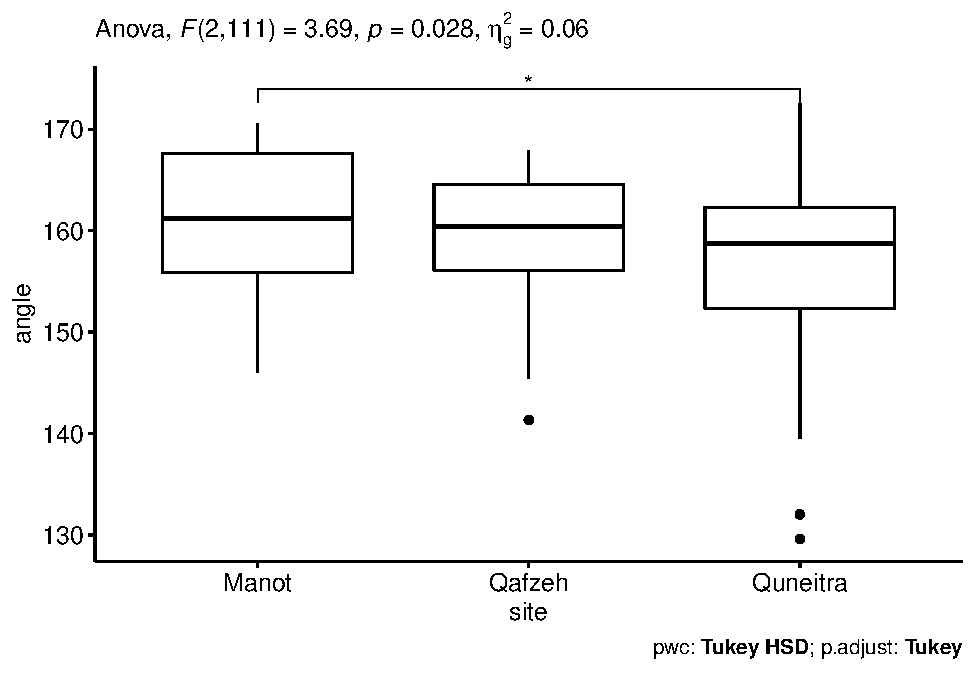
\includegraphics{incisionangles_files/figure-latex/unnamed-chunk-6-4.pdf}

\hypertarget{kruskal-wallis-test}{%
\section{Kruskal-Wallis test}\label{kruskal-wallis-test}}

\begin{Shaded}
\begin{Highlighting}[]
\NormalTok{ang.kruskal }\OtherTok{\textless{}{-}}\NormalTok{ db }\SpecialCharTok{\%\textgreater{}\%} \FunctionTok{kruskal\_test}\NormalTok{(angle }\SpecialCharTok{\textasciitilde{}}\NormalTok{ site)}
\NormalTok{ang.kruskal}
\end{Highlighting}
\end{Shaded}

\begin{verbatim}
## # A tibble: 1 x 6
##   .y.       n statistic    df      p method        
## * <chr> <int>     <dbl> <int>  <dbl> <chr>         
## 1 angle   114      6.24     2 0.0441 Kruskal-Wallis
\end{verbatim}

\begin{Shaded}
\begin{Highlighting}[]
\NormalTok{db }\SpecialCharTok{\%\textgreater{}\%} \FunctionTok{kruskal\_effsize}\NormalTok{(angle }\SpecialCharTok{\textasciitilde{}}\NormalTok{ site)}
\end{Highlighting}
\end{Shaded}

\begin{verbatim}
## # A tibble: 1 x 5
##   .y.       n effsize method  magnitude
## * <chr> <int>   <dbl> <chr>   <ord>    
## 1 angle   114  0.0382 eta2[H] small
\end{verbatim}

\begin{Shaded}
\begin{Highlighting}[]
\CommentTok{\# comparison between pairs}

\NormalTok{ang.will }\OtherTok{\textless{}{-}}\NormalTok{ db }\SpecialCharTok{\%\textgreater{}\%} 
  \FunctionTok{wilcox\_test}\NormalTok{(angle }\SpecialCharTok{\textasciitilde{}}\NormalTok{ site, }\AttributeTok{p.adjust.method =} \StringTok{"bonferroni"}\NormalTok{)}
\NormalTok{ang.will}
\end{Highlighting}
\end{Shaded}

\begin{verbatim}
## # A tibble: 3 x 9
##   .y.   group1 group2      n1    n2 statistic     p p.adj p.adj.signif
## * <chr> <chr>  <chr>    <int> <int>     <dbl> <dbl> <dbl> <chr>       
## 1 angle Manot  Qafzeh      37    22       437 0.646 1     ns          
## 2 angle Manot  Quneitra    37    55      1292 0.029 0.087 ns          
## 3 angle Qafzeh Quneitra    22    55       769 0.065 0.196 ns
\end{verbatim}

\begin{Shaded}
\begin{Highlighting}[]
\NormalTok{ang.will }\OtherTok{\textless{}{-}}\NormalTok{ ang.will }\SpecialCharTok{\%\textgreater{}\%} \FunctionTok{add\_xy\_position}\NormalTok{(}\AttributeTok{x =} \StringTok{"site"}\NormalTok{)}

\FunctionTok{ggboxplot}\NormalTok{(db, }\AttributeTok{x =} \StringTok{"site"}\NormalTok{, }\AttributeTok{y =} \StringTok{"angle"}\NormalTok{) }\SpecialCharTok{+}
  \FunctionTok{stat\_pvalue\_manual}\NormalTok{(ang.will, }\AttributeTok{hide.ns =} \ConstantTok{TRUE}\NormalTok{) }\SpecialCharTok{+}
  \FunctionTok{labs}\NormalTok{(}
    \AttributeTok{subtitle =} \FunctionTok{get\_test\_label}\NormalTok{(ang.kruskal, }\AttributeTok{detailed =} \ConstantTok{TRUE}\NormalTok{),}
    \AttributeTok{caption =} \FunctionTok{get\_pwc\_label}\NormalTok{(ang.will)}
\NormalTok{    )}
\end{Highlighting}
\end{Shaded}

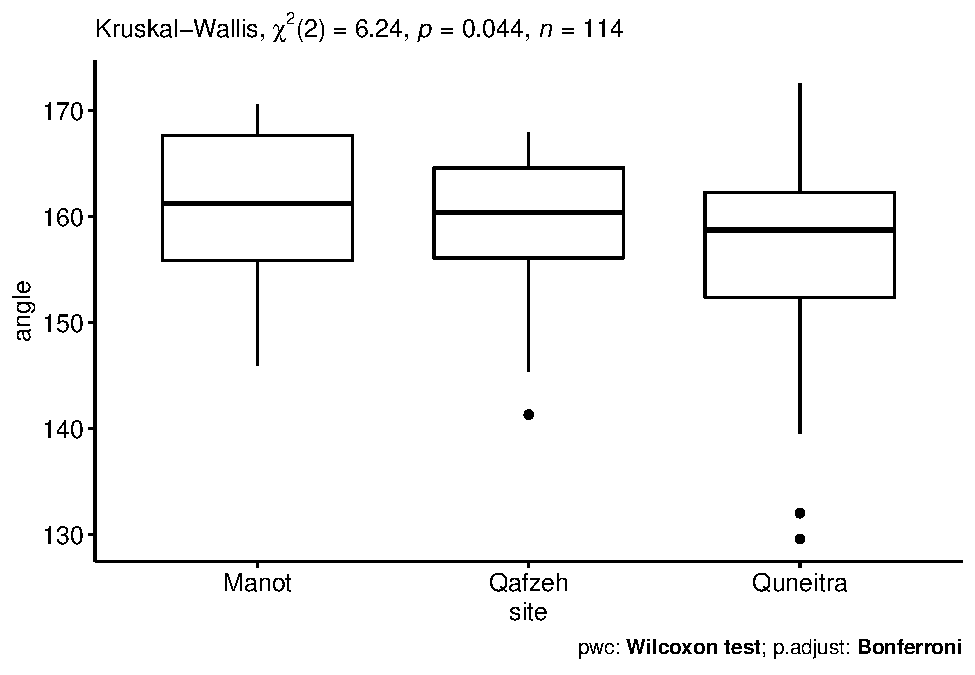
\includegraphics{incisionangles_files/figure-latex/unnamed-chunk-7-1.pdf}

\begin{Shaded}
\begin{Highlighting}[]
\FunctionTok{ggsave}\NormalTok{(}\StringTok{"../plots/anova.png"}\NormalTok{)}
\end{Highlighting}
\end{Shaded}

\begin{verbatim}
## Saving 6.5 x 4.5 in image
\end{verbatim}

\begin{center}\rule{0.5\linewidth}{0.5pt}\end{center}

End of Script

\end{document}
